%-*- coding: utf-8 -*-
\section{Ajax}
Ajax とは Asynchronous Javascript+XML の略で、非同期(Asynchronous)でWeb
ページとサーバーでデータの交換を行い、クライアント側で得られたデータをも
とにそのWebページを書き直す手法である\footnote{%
\texttt{http://adaptivepath.org/ideas/ajax-new-approach-web-applications/}}。
Google Maps がこの技術を利用したことで一気に認知度が高まった。検索サイト
では検索する用語の一部を入力していると検索用語の候補が出てくる。これも
Ajaxを使用している(と考えられる)。

Ajax の機能は \texttt{XMLHTTPRequest}というオブジェクトの機能を用いて実現されている。
\begin{Exec}\upshape\label{WhatDay}
次の例は実行例\ref{pulldownDate}で日付が変わったときに、その日の記念日を
 メニューの下部に示すものである。記念日のデータは
 \texttt{http://ja.wikipedia.org/wiki/日本の記念日一覧}の表示画面からコ
 ピーして作成した。
\LISTN{09-01whatday.html}{1}{last}{\normalsize}
\begin{itemize}
 \item 実行例\ref{pulldownDate}とは41行目以降が異なっている。
 \item イベントハンドラーを関数として定義している(41行目から60行目)。
 \item 42行目から48行目は以前と同じプルダウンメニューの処理である。
 \item 49行目では裏でサーバーと通信をするための
       \texttt{XMLHttpRequest}オブジェクトを作成している。
 \item \texttt{XMLHttpRequest}が生成できたら(50行目)、このオブジェクトの
       \texttt{onreadystatechange}イベントのイベントハンドラーを
       登録する(51行目から55行目)。
 \begin{itemize}
  \item \texttt{XMLHttpRequest}の\texttt{readyState}は通信の状態を表す。
	$4$ は通信終了を意味する。これらの値については表\ref{XMLHttpRequestRes}を参照
				のこと。
  \item 通信が終了しても正しくデータが得られたかを調べる必要がある。
	$200$ は正しくデータが得られたことを意味する\footnote{Http通信の終了
				コードについては
				\texttt{http://www.w3.org/Protocols/rfc2616/rfc2616-sec10.html}
				を参照のこと}。
  \item 得られたデータは\texttt{responseText}で得られる。この場合、得ら
	れたデータは文字列となる。このほかに\texttt{responXML}でXMLデー
	タが得られる。
 \end{itemize}
 \item 56行目から58行目が通信の開始部分である。ここでは、\texttt{GET}で行うので、
       URLの後に必要なデータを付ける。
 \item \texttt{GET}では送るデータ本体がないので、通信終了のため
       \texttt{null}を送信する。\texttt{POST}のときはここでデータ本体を
       送る。
 \item プルダウンメニューが変化したときのイベントハンドラーを登録し(62行
       目)、最後に現在の日付データをサーバーに要求する(63行目)。
 \item 得られたデータは69行目の\texttt{p}要素のテキスト
       (\texttt{innerText})として代入する(53行目)。
       %この要素の\texttt{firstChild}を指定しているので
       %\texttt{<p>}と\texttt{</p>}の間に空白を設けて、テキストノードが存
      % 在するようにしている。
\end{itemize}
 表\ref{XMLHttpRequestRes}の状態は\texttt{XMLHttpRequest}オブジェクトの
 プロパティである。たとえば、\texttt{XMLHttpRequest.DONE}で利用できる。
 \begin{table}[ht]
	\caption{XMLHttpRequestの通信の状態
\protect\footnote{\protect\texttt{https://developer.mozilla.org/ja/docs/Web/API/XMLHttpRequest}
	より引用}} \label{XMLHttpRequestRes}
		\begin{tabular}{|c|c|m{30zw}|}\hline
		 値&状態&\multicolumn{1}{c|}{詳細}\\\hline
		 0&\Verb+UNSENT+&\Verb+open()+ がまだ呼び出されていない。\\\hline
1&\Verb+OPENED+&\Verb+send()+ がまだ呼び出されていない。\\\hline
2&\Verb+HEADERS_RECEIVED+&\Verb+send()+ が呼び出され、ヘッダーとステータ
						 スが通った。\\\hline 
3&\Verb+LOADING+&ダウンロード中;\Verb+responseText+ は断片的なデータ
						 を保持している。\\\hline 
4&\Verb+DONE+&一連の動作が完了した。\\\hline
		\end{tabular}
 \end{table}
\input 17dev10-05.tex
 次のリストはAjaxで呼び出されるPHPのプログラムである。
\LISTN{aniversary.php}{1}{last}{\normalsize}
\begin{itemize}
 \item 2行目で内部で処理をするエンコーディングを\texttt{UTF8}にしている。
       関数、\texttt{mb\_internal\_encoding}関数を引数なしで呼び出すと
       現在採用されているエンコーディングを得ることができる。
 \item 4行目と5行目では月(\Verb+$m+)と日(\Verb+$d+)の値をそれぞれの変数
       に設定している。
\begin{itemize}
 \item ここではコマンドプロンプトからもデバッグで
       きるように、スーパーグローバル\Verb+$_GET+内に値があれば
       (\Verb+isset()+)が\Verb+true+になれば、その値を、そうでなければコ
       マンドからの引数を設定している。
 \item コマンドから実行したときの引数はスーパーグローバル\Verb+$argv+に
       格納される。一番目は呼び出したファイル名であ
       り、その後に引数が順に入る\footnote{C言語の\texttt{main}関数は通
       常、\texttt{int main(int argc, char* argv[])}と宣言される。%
       \texttt{argc}は\texttt{argv}の配列の大きさを表し、渡された引数の
       リストが\texttt{argv[]}に入っている。このとき、\texttt{argv[0]}は実行
       したときのファイル名が入る。}。
\end{itemize}
 \item 6行目の\texttt{file}関数は指定されたファイルを行末文字で区切って配
       列として返す関数である。この引数にはURLも指定できる。
\begin{itemize}
 \item この関数は2番目の引数をとることができる。次の定数を組み合わせて使
       う。
\begin{center}
 \begin{tabular}{|c|c|}\hline
 \Verb+FILE_USE_INCLUDE_PATH+ & \Verb+include_path+ のファイルを探す\\\hline
 \Verb+FILE_IGNORE_NEW_LINES+ & 配列の各要素の最後に改行文字を追加しない
      \\ \hline
  \Verb+FILE_SKIP_EMPTY_LINES+&空行を読み飛ばす \\ \hline
 \end{tabular}
\end{center}
 \item \Verb+file_get_contents()+はファイルの内容を一つの文字列として
       読み込む。Webページの解析にはこちらの関数を使うとよい。
\end{itemize}
 \item 読み込むファイルの一部を次に記す。
\begin{Verbatim}
1月[編集]
1日 - 鉄腕アトムの日
2日 - 月ロケットの日
[中略]
31日 - 生命保険の日、愛妻家の日
2月[編集]
1日 - テレビ放送記念日、ニオイの日
2日 - 頭痛の日
[以下略]
\end{Verbatim}
\begin{itemize}
 \item 月の部分の後には\texttt{[}がある。
 \item 日の情報は\Verb*+ - +で区切られている(\Verb*+ +は空白を表す)。
 \item すべての日の情報が入っている。
\end{itemize}
 \item 7行目から13行目までは指定された月の行を見つける。
\begin{itemize}
 \item 8行目で念のためコードを\texttt{UTF8}に変更している。
 \item 関数\Verb+mb_split()+関数は第1引数に指定された文字列パターンで第2
       引数で指定された文字列を分割して配列として返す関数である。
 \item 分割を指定する文字列には正規表現が使えるので、文字\Verb+[+で分割
       するために、\Verb+"\["+としている(9行目)。
 \item 指定された文字列があれば配列の大きさが1より大きくなる。その行に対
       して求める月と一致しているか判定し、等しければループを抜ける(11行
       目)。
\end{itemize}
 \item 14行目から18行目までは指定された月での指定された日の情報を探して
       いる。日を決定する方法も月と同じである。文字列の分割は
       \Verb+"\s-\s"+となっている\footnote{これは\texttt{"\textbackslash
       s"}ではうまく行かなかっ
       たためである。}。
 \item 20行目で得られた情報をストリームに出力している。
\end{itemize}
\end{Exec}
なお、構造化されたデータとしてはXML形式でもよいが、より軽量なJSONで与え
ることも可能である。このときは、\texttt{JSON.parse()}でJavaScriptのオブ
ジェクトに直せばよい。
\input 17dev10-06.tex

Ajax の通信で大きなデータを渡すためには\texttt{POST}で行う行う。この例
においては57行目から59行目の部分を次のように変更すれば\texttt{POST}で通
信できる。
\LISTN{09-01whatdayPOST.html}{57}{60}{\normalsize}
\begin{itemize}
 \item \ElmJ{open}メソッドの一番目の引数を\Verb+"POST"+に変更し、2番目の
			 引数を呼び出すURLにする。URLには\Verb+"GET"+のときのようにデータ
			 を記述しない。
 \item その後、\ElmJ{setRequestHeader}メソッドで\Verb+Content-type+を指定
			 する。
 \item その後、\Verb+send+メソッドで\Verb+GET+のときと同じ形式でデータを
			 送信する。
 \item 受け取る側のPHPのプログラムでは\Verb+$_GET+のところを
			 \Verb+$_POST+に変更する。
\end{itemize}
Ajax を用いてサーバーに同時に複数のデータを要求することも可能である。サー
バーがそれらの要求を並行処理するのであればデータ処理の効率化ができる
\footnote{PHPをサーバーモードで起動すると並行処理は行われないようである。
XAMPPでは並行処理が行われる。}。
\begin{Exec}\upshape\label{contPrimes}
 次のリストは$10,000,000$以下の素数を$1,000,000$ずつの区間に分けてサーバー
 に要求するものである。

 図\ref{countPrimes-Ajax-start}はこのWeb ページの初期画面である。
 \begin{figure}[ht]
	\begin{center}
	 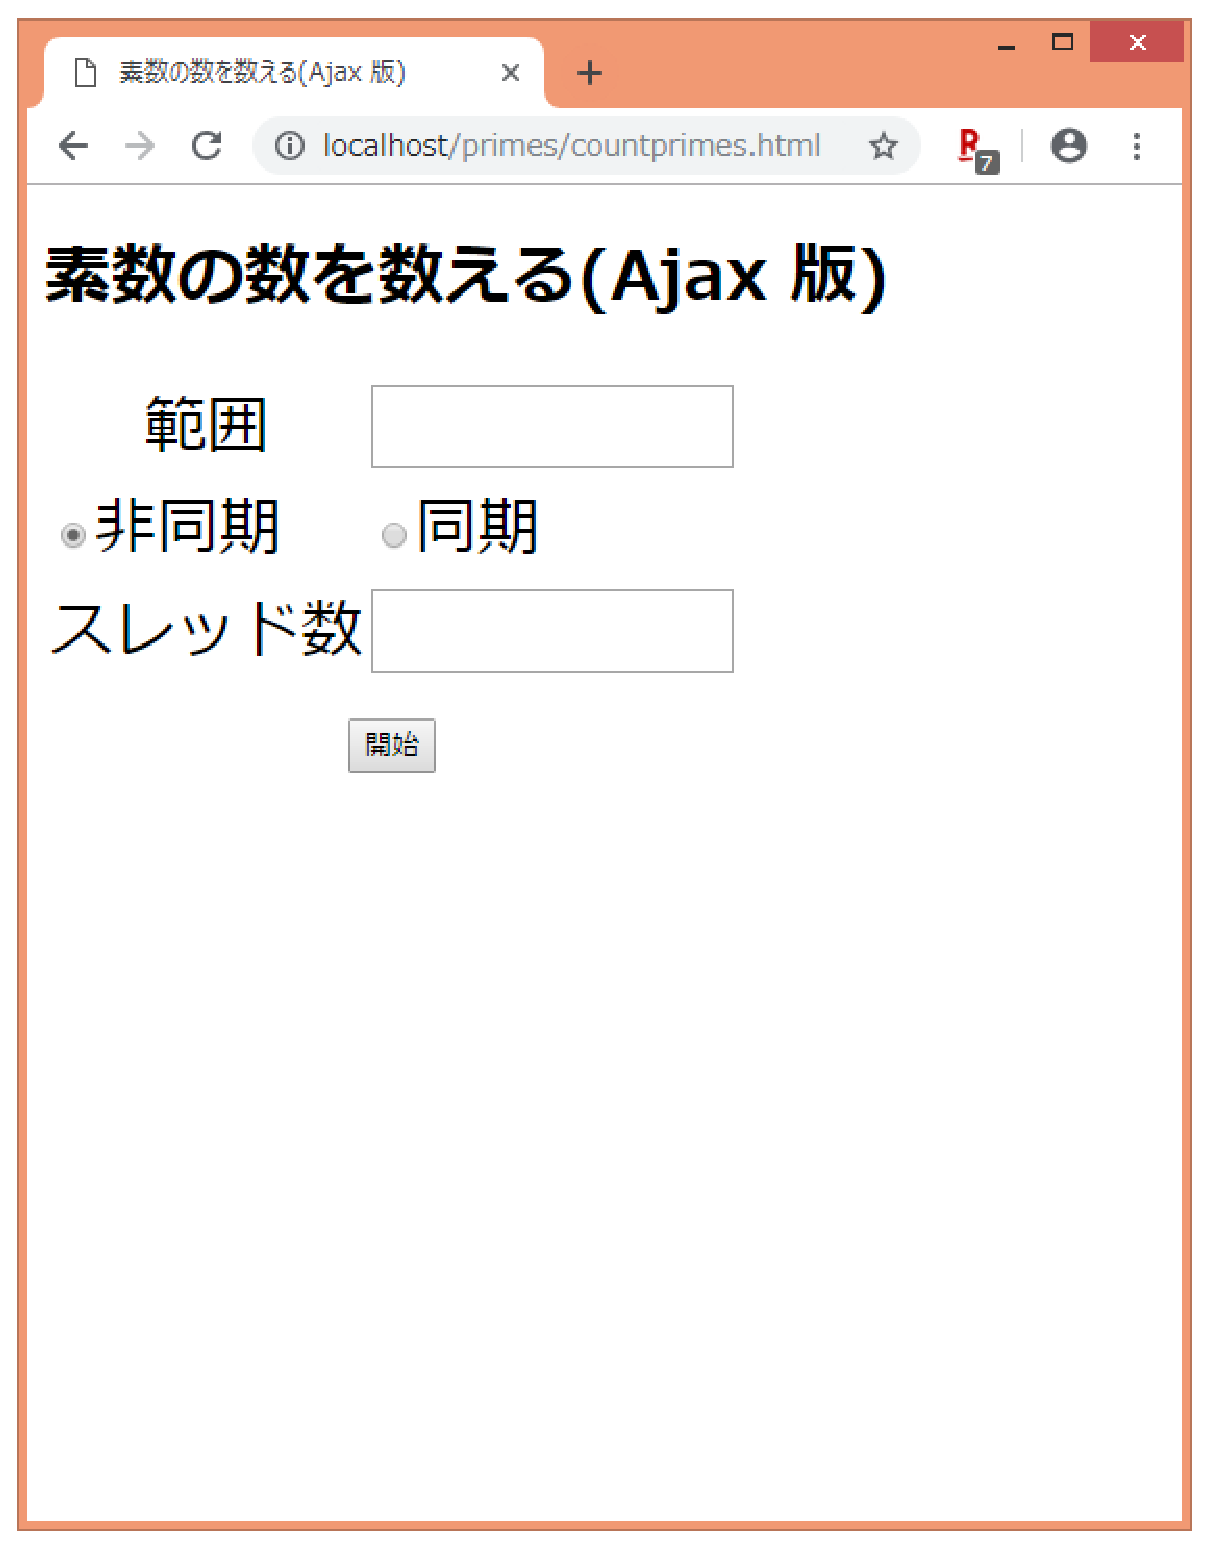
\includegraphics[width=0.5\textwidth]{primes/countPrimes-start.eps}
	\end{center}
 \caption{素数の数を数える(Ajax版)開始画面}\label{countPrimes-Ajax-start}
 \end{figure}

 素数の数を求める範囲と、Ajaxを実行するモード、求める区間の分割数と実行
 開始の美単が並んでいる。

図 \ref{countPrimes-Ajax-res}は求める範囲を$10,000,000$、分割を $10$に設
 定し、非同期モードで起動したことに結果画面である。
 \begin{figure}[ht]
	\begin{center}
	 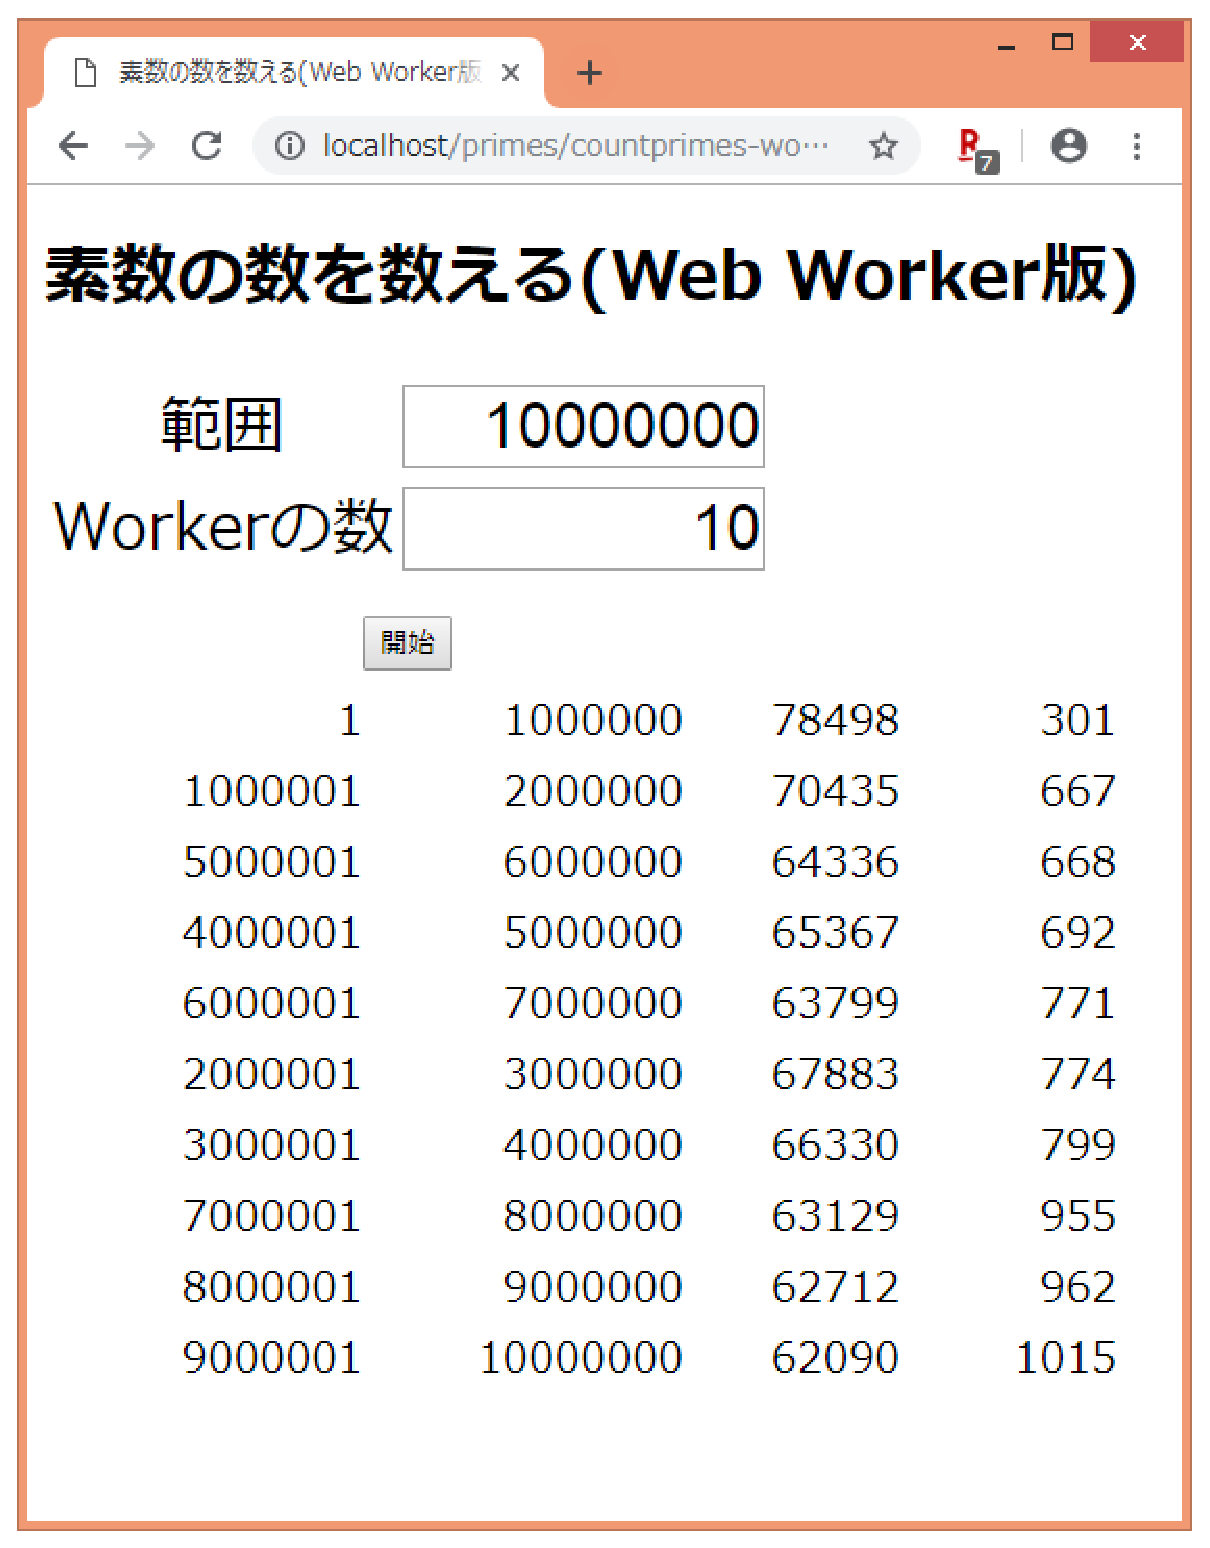
\includegraphics[width=0.5\textwidth]{primes/countPrimes-res.eps}
	\end{center}
 \caption{素数の数を数える(Ajax版)計算結果画面}\label{countPrimes-Ajax-res}
 \end{figure}

 項目は左から区間の下限と上限、その区間に含まれる素数の数、開始時間からその区間の実行
 終了までの時間(ミリ秒単位)である。
 
 次のリストは計算の起動と、結果を表示するWebページのものである。
 \LISTN{../primes/countPrimes.html}{1}{last}{\normalsize}
 \begin{itemize}
  \item 5行目で Ajax を用いてサーバーへの要求と結果を処理するJavaScriptっ
        ファイルを読み込む。
  \item 6行目でこのページに適用されるスタイルシートの読み込む。
  \item 13行目から16行目で素数の個数を求める範囲を指定するテキストボック
        スを配置している。
  \item 17行目から20行目でAjaxを起動するモードの指定をするラジオボタンを
        配置している。
  \item 21行目から24行目で同時に発行するAjaxの要求の個数を指定するテキストボック
        スを配置している。
  \item 25行目から29行目で計算開始するボタンを配置している。
 \end{itemize}
 次のリストは前のhtmlファイルで読み込まれるcssファイルの内容である。
 \LISTN{../primes/primes.css}{1}{last}{\normalsize}
 \begin{itemize}
  \item 1行目から4行目はテキストボックスに適用される。このページのテキス
        トボックスは数が入力さっるので、文字列を右寄せに(2行目)している。
  \item 5行目から7行目では\texttt{table}要素内の\texttt{td}要素の文字の
        大きさを指定している。 
  \item 8行目から12行目では素数の個数を表示する\texttt{table}要素ないの
        \texttt{td}要素の文字の位置(9行目)、文字の大きさ(10行目)と表示幅
        (11行目)を指定している。
  \item 13行目から15行目では右2つの\texttt{td}要素の幅を前の2つと異なる
        値に設定(\texttt{100px})している。
 \end{itemize}
 次のリストはAjaxを処理するためのJavaScriptファイルである。
 \LISTN{../primes/countPrimes-Ajax.js}{1}{last}{\normalsize}
 \begin{itemize}
  \item 2行目と3行目で\texttt{form}要素と結果を表示するための
        \texttt{table}要素を得ている。
  \item 4行目ではAjaxを非同期と同期モードの切り替えのラジオボタンを「非
        同期」に設定している。
  \item 6行目から44行目は「開始」ボタンが押されたときの処理を記述してい
        る。
        \begin{itemize}
         \item 6行目ではボタンの操作ができないようにしている。
         \item 7行目から9行目は結果を表示している内容を消去するために、
               表示する要素である\texttt{table}要素を取り除き(7行目)、そ
               の要素だけのコピー(子要素はなし)を作成(8行目)てそれを再び、
               子要素として登録(9行目)している。
         \item 10行目から11行目では素数を求める範囲を最低で$10^{6}$にな
               るようにしている。
         \item 12行目から13行目では区間を分ける数を設定している。
         \item 14行目では個々の処理で求める範囲の幅を求めている。
         \item 15行目ではその時点での時間を求めている。
         \item 16行目では発行したAjax通信の数を管理する変数を初期化して
               いる。
         \item 17行目から41行目で指定された個数分のAjax通信を発行してい
               る。
         \item 18行目から34行目ではAjax通信オブジェクトを作成している。
               作成が成功したのならば(35行目)発行した通信の数を一つ増や
               し(36行目)、通信を開始する(37行目から38行目)。
         \item 20行目から32行目はサーバーからのデータ処理の部分である。
         \item 20行目から21行目で表示1行分の要素\texttt{tr}を追加してい
               る。
         \item サーバーから送られてくるデータはJSON形式なのでそれを
               JavaScriptのオブジェクトに直し(22行目)ている。
         \item そのオブジェクトにボタンが押されてからの経過時間を追加(23
               行目)している。
         \item 24行目から28行目ではキーのリストを求め
               (\texttt{Object.keys()})、それらを順に\texttt{td}要素の中
               に表示している(25行目から27行目)。
         \item 28行目では発行したAjax通信の数を減らし、その値が$0$になっ
               たら「開始」ボタンが再び押せるようにしている
               (30行目から32行目)。
        \end{itemize}
 \end{itemize}
 次のリストはAjax通信で呼び出されるサーバー側のプログラムである。
 素数の判定は小さい素数で割り切れるかで行っている\footnote{ここでは非同期で処理
 が行われる例を出すために、素数の判定に関しては単純な方法を採用している。
 エラトステネスの篩を用いると処理速度は向上する。}。
 \LISTN{../primes/countPrimes.php}{1}{last}{\normalsize}
 \begin{itemize}
  \item PHPファイルをコマンドプロンプトからデバッグできるように、処理の
        ためのパラメータの処理を行っている(2行目と3行目)。スーパーグロー
        バル変数\Verb+$_GET+に指定したキーがあればそれを使用し、なければ
        コマンドラインの引数を格納する変数\Verb+$argv+をその値としている。
  \item 4行目では保存する素数の上限の値を設定し、その値を変数
        \Verb+$primes+に配列として格納する。この変数は5行目で初期化され
        ている。
  \item 6行目から15行目で残りの素数を求めている。ある数\Verb+$i+がその数
        の平方根以下の素数で割り切れないのならば素数と判定できる(10行目)。
  \item 16行目以下が与えられた区間における素数の個数を求める部分である。
  \item 開始の値が小さい場合には\Verb+$limit+以降から探し、素数の個数を
        \Verb+count($primes)+に初期化する(18行目から21行目)。
  \item 開始の値を奇数に設定し(22行目)、最後の値を求める(23行目)
  \item 26行目から35行目で与えられた区間の奇数が素数であるかの判定を行っ
        ている。この部分は小さい素数を求める部分と同じアルゴリズムである。
  \item 17行目、24行目36行目でクライアント側に送るデータを作成している。
  \item 37行目ではその結果をJSON形式に変換して、クライアント側に送ってい
        る。
 \end{itemize}
\end{Exec}
\section{Web Worker}
ブラウザにおけるJavaScriptの処理はどこか一か所しか実行されない。これによ
りあるイベントが処理されている間は他のイベントの処理が行われないのでプロ
グラムのアルゴリズムが簡単になる。一方、最近のCPUではマルチコアが標準と
なり、複数の処理を同時に行うことは当たり前となっている。

並行処理を行う方法としては独立したプログラム(プロセス)を用いる方法と、単一のプログ
ラム内でスレッドと呼ばれる実行単位を起動して行う方法がある。
独立したプログラムで行う場合にはそれぞれのプログラムがデータを個別に持つ
ので共通のデータを必要な時に渡したり、参照し
たりする機能を効率よく行う必要がある。

一方、スレッドはあるプログラム内で起動され、元のプログラムと同じメモリーっ
空間を共有するために、データの受け渡しをしなくてもよい。

ブラウザにおける
JavaScriptで並行処理を行う機能を提供するものとしてWeb Workerオブジェクト
が提案されている
\footnote{\texttt{https://developer.mozilla.org/en-US/docs/Web/API/Web\_Workers\_API/Using\_web\_workers}\label{webworkers}}
。
Workerオブジェクトは呼び出されるプログラムとは別のメモリー空間で実行され、
元のプログラムとのデータ交換はメッセージの通知というイベントを通じて行う。

この節では前節の素数の数を求めるプログラムをWeb Worker を用いて書き直し
 たものを紹介する。

 なお、このプログラムをエクスプローラーからダブルク
 リックして起動する(URLが\texttt{file:}で始まる)と、ブラウザによって
 は\texttt{Worker}が起動できないことがある。その場合にはローカルにサーバー
 を起動し、必要なファイルをドキュメントルートにコピーすればよい。
 \pageref{webworkers}ページの脚注\ref{webworkers}にあるブラウザに関する互換
 性の部分を参照のこと。

   \begin{Exec}\upshape
    図\ref{countPrimes-workers-res}はWeb Workers を利用して素数を求める
    Webページの結果画面である。
    \begin{figure}[ht]
	\begin{center}
	 \includegraphics[width=0.5\textwidth]{primes/countPrimes-workers-res.eps}
	\end{center}
 \caption{素数の数を数える(Web workers版)計算結果画面}\label{countPrimes-workers-res}
 \end{figure}

    計算結果の順がばらばらで、計算速度も速いことが分かる。
    
 次のリストはWeb Worker版の素数の数を求めるHTMLファイルである。
 \LISTN{../primes/countPrimes-workers.html}{1}{last}{\normalsize}
 以前のも のからラジオボタンの部分がないものとなっている。当然のことなが
 ら読み込まれるJavaScriptファイルも異なっている。

 次のリストは読み込まれるJavaSCriptファイルである。
 \LISTN{../primes/countPrimes-workers.js}{1}{last}{\normalsize}
 Ajax通信のときと比較できるようにできるだけ同じプログラムの流れとなって
 いる。
 \begin{itemize}
  \item 13行目まではAjaxのときと同じである。
  \item 17行目から20行目で必要な個数のWeb Workerオブジェクトを作成してい
        る。Web Workerオブジェクトは\Verb+Worker+コンストラクタで作成す
        る。この引数には処理をするJavaScriptファイルを指定する。
  \item Workerオブジェクトにデータを送るメソッドが\ElmJ{postMessage}であ
        る。引数としてはJavaScriptで扱えるデータを用いる。ここではオブジェ
        クトを与えている。
  \item Workerからのメッセージは\Verb+onmessage+イベントを通じて受け取る
        ことができる。この引数は\Verb+message+オブジェクトであり、その
        \Verb+data+プロパティが送られてきたデータとなる(26行目)。
  \item データが送られてきたので\Verb+worker+の動作を停止し(35行目の
        \Verb+terminate+メソッド)、オブジェクトを消去する(36行目)。
 \end{itemize}
 \Verb+worker+オブジェクトに再びメッセージを送れば再度処理をさせることが
 できる。

 次のリストは\Verb+worker+の処理をするJavaScriptのプログラムである。
 \LISTN{../primes/primes.js}{1}{last}{\normalsize}
 \begin{itemize}
  \item 1行目の\Verb+self+は\Verb+Worker+のもととなるオブジェクトを指す。
        こので\Verb+onmessage+イベントの処理のプログラムを登録する。
  \item 処理内容は全く前と同じである。workerが2回目以降呼び出されたかど
				うかを記憶する変数(2行目の変数\texttt{Status})を利用して2回目以
				降の呼び出し時には素数のリストを再度作成しないようにするためにい
				くつかの変数をイベント処理関数の外で定義している(1行目から3行目)。
  \item 最後に\ElmJ{postMessage}メソッドを用いて呼び出し元にデータを送信
        する(39行目から40行目)。
 \end{itemize}
\end{Exec}
 \begin{Prob}\upshape このリストについて次のことを行いなさい。
  \begin{enumerate}
   \item 実行するごとに結果の並びや計算終了時間が変化すること。
   \item スレッドの個数を変えると表示する区間が変化すること。また、どの
         場合が一番実行時間が短いかを調べる。
   \item 計算結果が戻ってきた順に区間の上限と下限やその
 区間の素数の個数が表示される。素数の区間が小さい方から大きい方に並ぶよ
 うにプログラムを直す。
   \item 同時に起動する\texttt{worker}の数を減らして、一つの処理が終わっ
         た時に別の区間の処理を与えるようにプログラムを直す。たとえば、区間は10に
         分けるが、生成する\texttt{worker}は3つにするように指定でき
         るようにする。
  \end{enumerate} 
 \end{Prob}